%%==================================================================%%
%% Author : Perelló Nieto, Miquel                                   %%
%% Version: 1.0, 04/11/2011                                         %%
%%                                                                  %%
%% Memoria del Projecte de Final de Carrera                         %%
%% Disseny del laboratori                                           %%
%%==================================================================%%

\chapter{Disseny del laboratori}\label{cap:dis}


% the code below specifies where the figures are stored
\ifpdf
    \graphicspath{{3_laboratory_design/figures/PNG/}{3_laboratory_design/figures/PDF/}{3_laboratory_design/figures/}}
\else
    \graphicspath{{3_laboratory_design/figures/EPS/}{3_laboratory_design/figures/}}
\fi


% ----------------------- contents from here ------------------------

Aquest capítol comença amb l'explicació de l'entorn i dels objectius que té el laboratori actual de Sistemes de Control Empotrats i en Xarxa. Exposarem per tant el seu proposit i les limitacions que aquest tenía, i de quina manera hem dissenyat la nova plataforma per poder solventar algunes d'aquestes mancanses.
Per tant entrarem en la part del disseny del nou laboratori, i veurem les raons que ens han portat a escollir els diferents camins que teniem, així com el disseny de les comunicacions que hi ha entre els diferents dispositius i el nou programa \DCSMonitor.

%====================================================================================%
% Laboratori actual
%====================================================================================%
\section{Resum del laboratori actual}\label{cap:dis:resum}

L'objectiu d'aquest laboratori és l'analisis, el diseny i la implementació d'un sistema de control empotrat i en xarxa (a partir d'ara \NECS, sigles de l'anglès Networked and Embedded Control Systems) \cite[laboratori complert en el document \emph{Networked and Embedded Control Systems (NECS) Double Integrator Control Lab}]{NECSDoubInt}.

En aquest laboratori es cobreixen varies fases:

\begin{itemize}
	\item Disseny de controls.
	\item Anàlisis de sistemes \NECS multitasques.
	\item Diseny de sistemes \NECS multitasques.
	\item Implementació del sistema \NECS.
\end{itemize}

La plataforma d'implementació ens permetrà controlar un circuit Doble Integrador (a partir d'ara \DI de l'anglés Double Integrator) d'un microcontrolador. Com es mostra en les figures \ref{microprocessor_based_control} i \ref{network_based_control}.

\figuremacroW{microprocessor_based_control}{Microprecessor-based control}{}{0.35}

\figuremacroW{network_based_control}{Network-based control}{}{0.6}

En la primera configuració, figura \ref{microprocessor_based_control}, moltes tasques són executades concurrentment al cap davant del Sistema Operatiu en Temps Real Erika. Per aquesta raó les tasques de control del circuit doble integrador han de competir amb la resta per el temps de CPU.

En la segona configuració, figura \ref{network_based_control}, permet tancar el llaç de control en una xarxa, en aquest cas un bus CAN. En aquest escenari, les limitacions dels recursos ve donada per l'ampla de banda de la comunicació. D'aquesta manera connectant varis llaços en una mateixa xarxa ens pot permetre analitzar un sistema distribuït de control més realista.

En les dues configuracions, les plaques estan equipades amb microcontroladors dsPIC33FJ256MC710 de \Microchip. Les plaques són plaques \FLEX de Evidence. S'han creat tres plaques amb un circuit doble integrador (figura \ref{DI_down}), comunicació CAN (figura \ref{DI_up})i un port RS232 (figura \ref{RS232_up}) que s'han afegit a aquestes per tal de comunicar-se entre elles, i amb l'ordinador.

\begin{figure}[ht!]
	\begin{center}
		\subfloat[Doble Integrador]{\label{DI_down}
			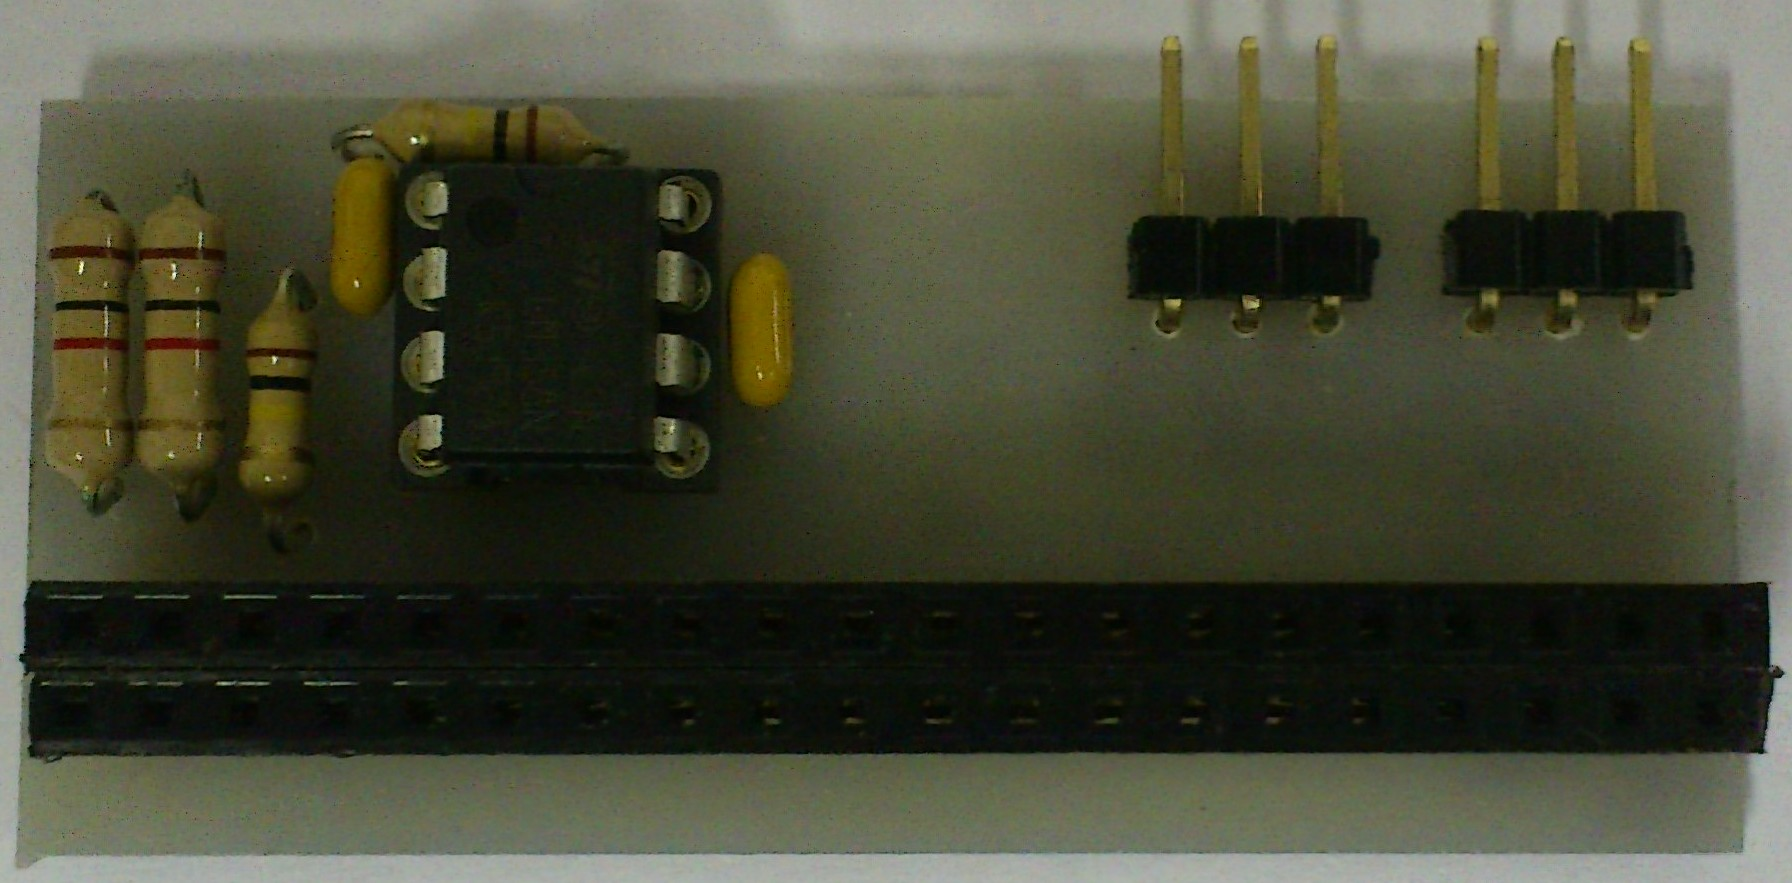
\includegraphics[width=0.4\textwidth]{DI_down}
		}
		\subfloat[Transceptor CAN]{\label{DI_up}
			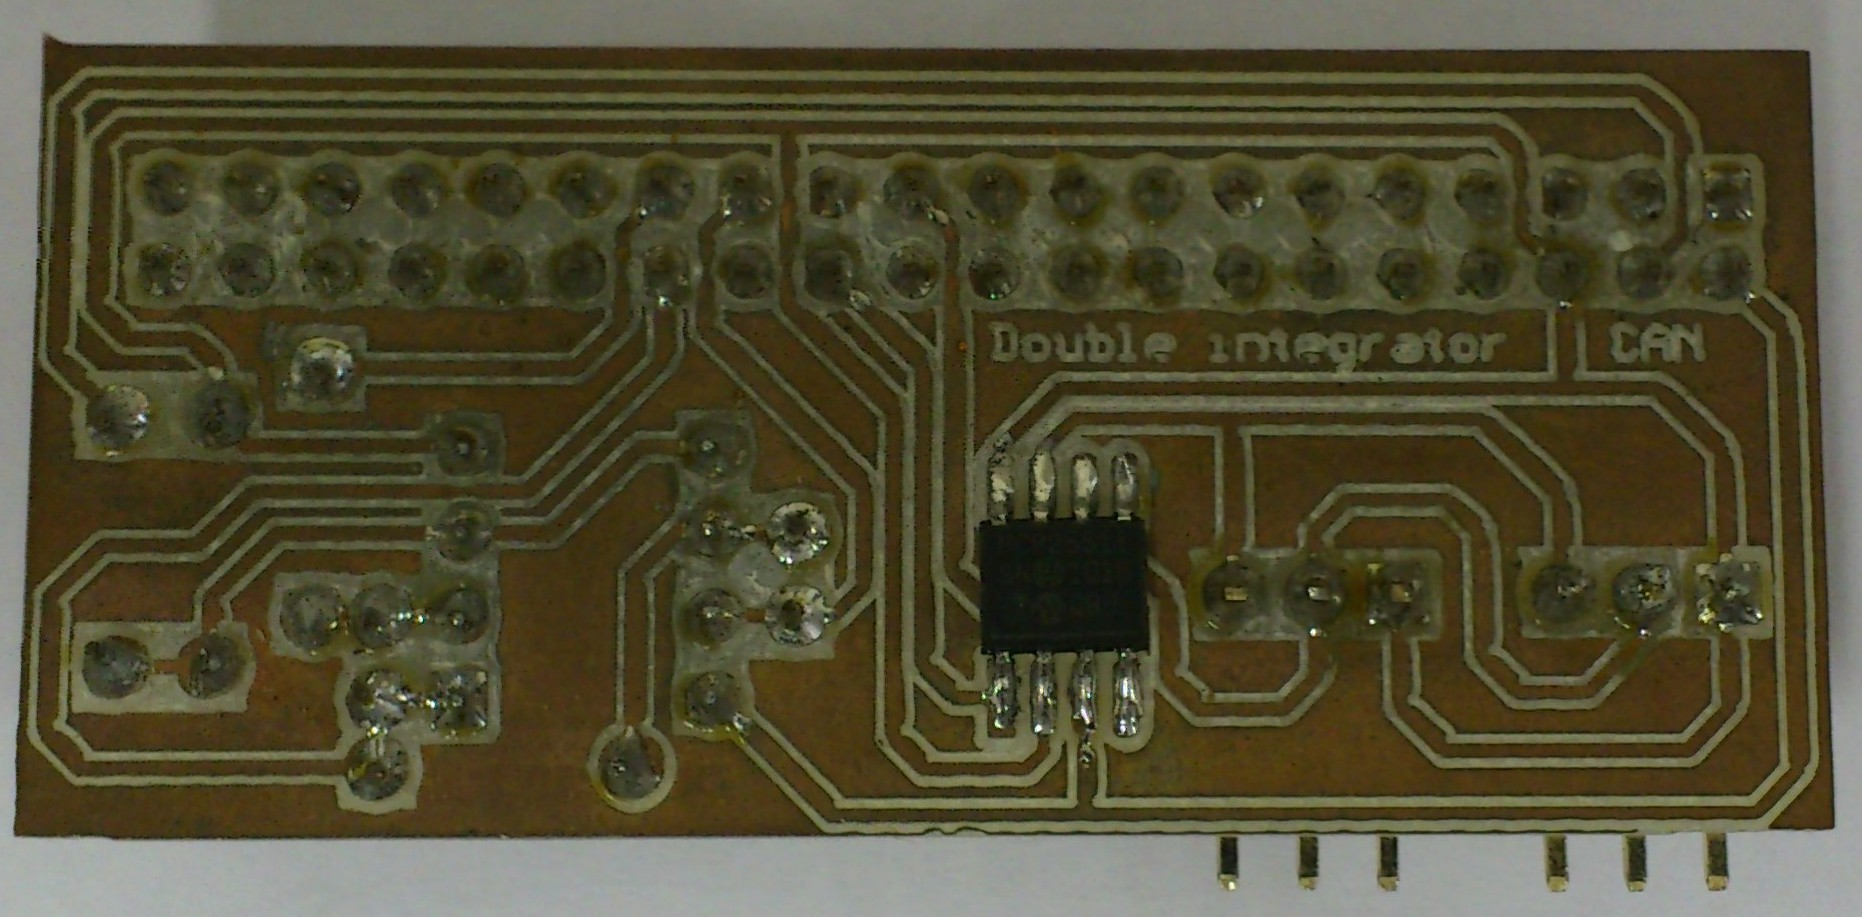
\includegraphics[width=0.4\textwidth]{DI_up}
		}

		\subfloat[Modul RS232]{\label{RS232_up}
			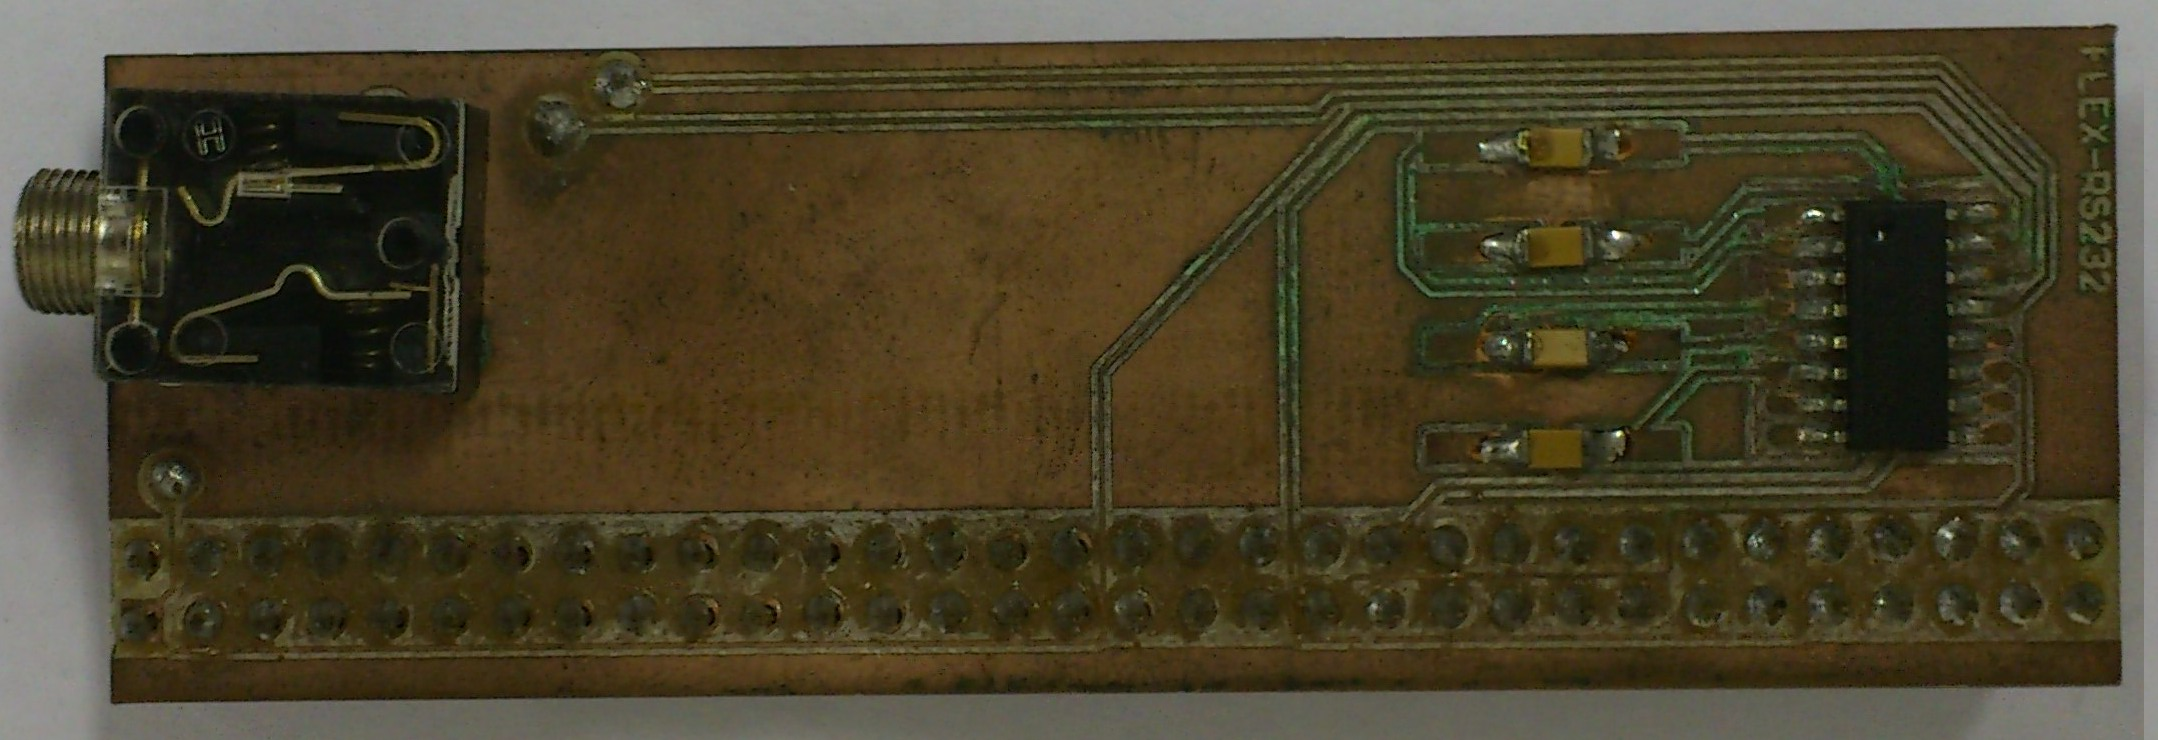
\includegraphics[width=0.6\textwidth]{RS232_up}
		}
	\end{center}
	\caption{Periferics per les plaques \FLEX.}
    \label{fig:plaques}
\end{figure}

La placa \FLEX que porta el circuit doble integrador es l'encarregada de simular un \Sensor i un \Actuador, en els quals el \Sensor es un conversor analogic digital (ADC) que llegeix els voltatges de sortida de la primera i segona integral, i l'\Actuador aplica diferents nivells de voltatge a l'entrada del circuit a través d'un modulador per amplada de polsos (PWM).

L'objectiu del control es que la sortida del doble integrador segueixi un valor de referencia que va variant. Aquest s'aconsegueix aplicant un algoritme de control i aplicant el valor calculat a l'entrada del circuit.

Un cop l'entorn està preparat la configuració queda com a la figura \ref{DCS_NECS_SCA_diagonal}. En la qual la placa superior actua com a \Controlador que remotament fa el control a traves del bus CAN. En la part inferior tenim el \SensorActuador que compta amb la placa del doble integrador connectada, i per tal de debugar el control també compta amb la interfície RS232 (en aquesta imatge queda sota de la placa superior) la qual envia periòdicament els valors de l'estat.


\figuremacroW{DCS_NECS_SCA_diagonal}{Llaç de control}{}{0.5}



%====================================================================================%
% Nou laboratori
%====================================================================================%
\section{Disseny del Nou laboratori}\label{diss:nou}

Fins aquest moment els problemes a resoldre han estat pels temps de demora que hi havia entre lectures del \Sensor, accions de l'\Actuador i els càlculs que havia de fer el \Controlador.

En aquest apartat ens interessa que tots els dispositius estiguin en un mateix bus CAN i comprovar el funcionament dels llaços en un entorn compartit, amb diferents tipus de prioritats i amb la possibilitat de saturar el bus en certes ocasions.

A part d'aquesta connexió general al bus, també s'introduirà en la xarxa un dispositiu que anomenarem \Monitor, el qual tindrà la opció de monitoritzar tots els paquets de dades d'un cert llaç de control (un grup format per un \Sensor, un \Actuador i un \Controlador).

Tota la informació que el nou dispositiu \Monitor capturi, podrà ser enviada mitjançant el port sèrie RS232 a un programa d'ordinador (\DCSMonitor) el qual mostrarà mitjançant unes gràfiques en temps real l'estat del control de cada grup del laboratori.

A més el \Monitor tindrà la capacitat d'incrementar la carrega del bus en quant a nombre de missatges CAN que hi circulin, dificultant el correcte funcionament dels llaços, i podent comprovar en temps real la resposta d'aquests.

Amb aquesta idea general i tenint en compte les relacions que hi haurà entre tots els elements que formen el laboratori es va dissenyar un esquema general en el que apareixen aquests elements i el tipus de comunicació que hi ha entre ells (figura \ref{esquema_general_v8}).
% El diagrama de comunicacions ocupa una pagina sencera, i està posicionat horitzontalment, amb aquest ifthenelse el diagrama sempre es mirarà desde la part exterior del llibre, rotant el diagrama 180 graus si cal.
%\ifthenelse {\isodd{\thepage}}
%{
%\figuremacroWR{esquema_general_v8}{Diagrama general dels elements del laboratori}{Diagrama de tots els elements que formen part del laboratori, i les diferents comunicacions que els relacionen.}{1}{180}
%}
%{
%\figuremacroW{esquema_general_v8}{Diagrama general dels elements del laboratori}{Diagrama de tots els elements que formen part del laboratori, i les diferents comunicacions que els relacionen.}{1}
%}

\begin{landscape}
\figuremacroWR{esquema_general_v8}{Diagrama general dels elements del laboratori}{Diagrama de tots els elements que formen part del laboratori, i les diferents comunicacions que els relacionen.}{1}{270}
\end{landscape}
%\figuremacroW{comunicacio_pc_monitor_v6}{Diagrama de comunicacions i identificadors}{Diagrama de funcionament del laboratori, disseny dels identificadors i màscares per bus CAN, i tipus de missatges de comunicació.}{1}

%====================================================================================%
% Interficie
%====================================================================================%
\subsection{Interficie}\label{cap:dis:visual}

Aquest programa es només una eina per visualitzar i comprovar el funcionament dels diferents controls que hi hagin al bus CAN, o el control del llaç al que estigui connectat, però en cap moment ha de ser un programa complicat d'executar, ja que el seu objectiu principal es precisament ajudar en aquesta tasca. Això implicava que el programa fos senzill d'utilitzar, però a l'hora complert.

Primer de tot calia saber quines opcions havien d'aparèixer a primera vista, així que es va fer un llistat d'elements necessaris:

\begin{itemize}
	\item Llista dels identificadors dels diferents controls al bus CAN
	\item Estat del port sèrie RS232
	\item Lectures dels valors del control en format text
	\item Gràfica del control
	\item Mostrar/eliminar dades de la gràfica
		\begin{itemize}
			\item Referència
			\item Valor d'entrada
			\item Primera integral
			\item Segona integral
		\end{itemize}
	\item Idioma per seleccionar
		\begin{itemize}
			\item Català
			\item Espanyol
			\item Anglès
			\item Francès
		\end{itemize}
	\item Mode de comunicació
		\begin{itemize}
			\item Comunicant amb \SensorActuador
			\item Comunicant amb \Monitor
		\end{itemize}
	\item Dades informatives (extres)
		\begin{itemize}
			\item Total de llaços de control al bus CAN
			\item Imatges per segon mostrades en la gràfica en temps real
			\item Nombre de mostres de cada línia de la gràfica
			\item Bytes pendents en el buffer d'entrada del port sèrie RS232
			\item Algun ítem intermitent que indiqui que les dades s'actualitzen correctament (en temps real)
		\end{itemize}
	\item Botó per connectar al port sèrie
	\item Botó per llistar llaços del bus CAN
	\item Botó per guardar una imatge de la gràfica
	\item Botó per netejar el text
	\item Botó per començar i aturar la monitorització
\end{itemize}

Un cop remarcats aquests elements, només calia identificar aquells que havien de ser accessibles directament, i posicionar-los de tal manera que fos intuïtiu d'utilitzar. Per tant es va treure la selecció d'idioma i de mode d'execució de la pantalla principal i es va posar en les \emph{Preferències} del programa, de la mateixa manera amb el mode d'execució del programa ja que els alumnes sempre faran servir el mode \SensorActuador i el professor el mode \Monitor.

Abans de començar a dissenyar la interfície amb algun programa d'edició, es van fer alguns esbossos de com hauria de quedar la organització, i finalment es va decantar pel dibuix de la figura \ref{esquema_interficie}.

\figuremacroWR{esquema_interficie}{Esquema de la interfície del programa \DCSMonitor}{}{0.6}{270}

Ja amb l'esquema ben clar es van provar varis IDE's d'edició d'interfície, i un cop analitzades varies qüestions es va decidir utilitzar \QTCreator. Aquestes són algunes de les raons que em van fer decantar per aquest IDE:

\begin{itemize}
	\item Existencia de bona documentació de les API's de QT.
	\item Portabilitat a altres sistemes operatius com Windows.
	\item Un entorn molt intuïtiu.
	\item Fàcil integració amb widgets propis.
	\item Existencia d'exemples d'integració de matplotlib amb QT4 \cite[Capítol 6 del llibre \emph{Matplotlib for Python Developers}]{EmbedMatQT4}
\end{itemize}

%====================================================================================%
% Identificadors dels missatges CAN
%====================================================================================%
\subsection{Identificadors dels missatges CAN}\label{cap:dis:idCAN}

El primer problema que hem de resoldre al dissenyar un sistema distribuït en el qual hi haurà múltiples dispositius és enviar i rebre els diferents missatges al dispositiu indicat.

En el laboratori anterior existien 3 tipus de missatge diferents (s'han mantingut els noms originals):
\begin{enumerate}
	\item \textbf{Sensor to controller message}
	
		Aquest missatge l'enviava el \Sensor i anava destinat al 
		\Controlador, i portava el primer i el segon valor de sortida 
		del doble integrador.
	\item \textbf{Controller to actuator message}
	
		Aquest missatge el generava el \Controlador i anava destinat
		al \Actuador, el seu contingut eren 4 Bytes amb el valor 
		d'entrada del doble integrador.
	\item \textbf{Controller updates reference (supervision)}
	
		Aquest missatge generat pel \Controlador tenia com a destinació el
		supervisor (\SensorActuador) i contenia el valor de referència
		teòric que hauria de seguir el doble integrador.
\end{enumerate}

Els identificadors per aquests tres missatges eren senzills de proposar ja que tenien els 29 bits de l'identificador per escollir sense cap tipus de restricció, per aquest motiu els missatges de control, estat del sensor i referenica podien tenir els identificadors 1, 2, i 3 respectivament. Cada dispositiu conneixia l'identificador del senyal que volia i per tant podia rebre aquests senyals.

En el disseny actual es volia introduir un entorn compartit, per tant hem dividit l'identificador de missatge CAN en subparts, per tal d'afegir noves funcionalitats:

 \begin{itemize}
 	\item Diferents nivells de prioritat.
 	\item Diferents identificadors de llaços de control.
 	\item Diferents classes de missatge.
 	\item Diferents subclasses de missatge. 
 \end{itemize}

Així que s'ha dissenyat un sistema d'identificadors per tal de complir tots aquests requisits. A més per tal de garantir els temps de resposta dels controladors i el millor funcionament del control s'ha procurat seguir el disseny realitzat a l'article "Schedulability Analysis for CAN-based Networked Control Systems with Dynamic Bandwith Management" \cite{SchAnaCANbasNCS}. 

En la figura \ref{fig:bit_encoding} es pot veure la codificació que es va seguir en l'article en el que es van fer els càlculs per garantir un funcionament òptim del control (s'ha mantingut el text original).

% ---------------------- Dibuix d'identificadors CAN -------------------------

\begin{figure}[ht!]
	\subfloat[Control message]{\label{fig:cont}
		\begin{bytefield}[bitwidth=\linewidth/29]{29}
			\bitlabel{3}{3 bits} \bitlabel{16}{16 bits} \bitlabel{8}{8 bits} \bitlabel{2}{2 bits} \\
		    \bitheader{0,2,3,18,19,26,27,28} \\
		    \bitbox{1}{0} \bitbox{1}{0} \bitbox{1}{0}  \bitbox{16}{Control signal} \bitbox{8}{ID} \bitbox{2}{\color{lightgray}\rule{\width}{\height}}
		\end{bytefield}
	}
	
	\subfloat[Granted sensor messages]{\label{fig:grant}
		\begin{bytefield}[bitwidth=\linewidth/29]{29}
			\bitlabel{3}{3 bits} \bitlabel{16}{16 bits} \bitlabel{8}{8 bits} \bitlabel{2}{2 bits} \\
		    \bitheader{0,2,3,18,19,26,27,28} \\
		    \bitbox{1}{0} \bitbox{1}{0} \bitbox{1}{1} \bitbox{16}{Error value} \bitbox{8}{ID} \bitbox{2}{\color{lightgray}\rule{\width}{\height}}
		\end{bytefield}
	}
	
	\subfloat[General purpose message]{\label{fig:general}
		\begin{bytefield}[bitwidth=\linewidth/29]{29}
			\bitlabel{3}{3 bits} \bitlabel{26}{26 bits} \\
		    \bitheader{0,2,3,28} \\
		    \bitbox{1}{0} \bitbox{1}{1} \bitbox{1}{0}  \bitbox{26}{Rest of applications}
		\end{bytefield}
	}
	
	\subfloat[Best effort sensor message]{\label{fig:best}
		\begin{bytefield}[bitwidth=\linewidth/29]{29}
			\bitlabel{3}{3 bits} \bitlabel{16}{16 bits} \bitlabel{8}{8 bits} \bitlabel{2}{2 bits} \\
		    \bitheader{0,2,3,18,19,26,27,28} \\
		    \bitbox{1}{0} \bitbox{1}{1} \bitbox{1}{1} \bitbox{16}{Error value} \bitbox{8}{ID} \bitbox{2}{\color{lightgray}\rule{\width}{\height}}
		\end{bytefield}
	}
	
    \caption[Codificació de bits dels identificadors CAN per tipus de missatges]{ Codificació de bits dels identificadors CAN per tipus de missatges - usats en l'article "Schedulability Analysis for CAN-based Networked Control Systems with Dynamic Bandwith Management" \cite{SchAnaCANbasNCS} (text original).}
    \label{fig:bit_encoding}

\end{figure}

Un cop revisat el funcionament d'aquests identificadors i dels missatges que en el nostre laboratori havíem de generar, es va pensar en la millor reorganització que es podia fer dels nostres missatges, i finalment va quedar el següent esquema genèric per tots els missatges (figura \ref{fig:bit_encoding:CAN:nou:generic}).

\begin{figure}[ht!]
	\begin{bytefield}[bitwidth=\linewidth/29]{29}
		\bitlabel{3}{3 bits} \bitlabel{16}{16 bits} \bitlabel{8}{8 bits} \bitlabel{2}{2 bits} \\
	    \bitheader{0,2,3,18,19,26,27,28} \\
	    \bitbox{3}{Tipus} \bitbox{16}{Prioritat} \bitbox{8}{ID llaç} \colorbitbox{lightgray}{2}{XY}
	\end{bytefield}
    \caption{Esquema genèric dels identificadors CAN pel nou laboratori.}
    \label{fig:bit_encoding:CAN:nou:generic}
\end{figure}

Aquest esquema ens permet adaptar tots els missatges que hi havia fins ara, i a més podem generar nous missatges utilitzant l'identificador de tipus genèric de 3 bits (010) utilitzant els últims dos bits per indicar quin missatge és.

Amb tots aquests punts ben clars es va crear un diagrama dels elements que formaran el laboratori, amb tots els dispositius que poden formar part d'ell, i les diferents interaccions que han de realitzar. En aquest diagrama podrem observar els períodes dels diferents missatges, l'esquema d'identificadors i el tipus de màscares i filtres que seran útils per rebre els missatges. Tot això es pot observar en el diagrama de la figura \ref{comunicacio_can_v8}.

% El diagrama de comunicacions CAN ocupa una pagina sencera, i està posicionat horitzontalment, amb aquest ifthenelse el diagrama sempre es mirarà desde la part exterior del llibre, rotant el diagrama 180 graus si cal.
\begin{landscape}
\figuremacroWR{comunicacio_can_v8}
{Diagrama de comunicacions i identificadors CAN}{Diagrama de funcionament del laboratori, disseny dels identificadors i màscares per bus CAN, i tipus de missatges de comunicació.}{1}{270}
\end{landscape}

Tot seguit es veuran un a un tots els missatges que s'han adaptat i creat explicats a fons.


%====================================================================================%
% Missatge de control per l'Actuador
%====================================================================================%
\subsubsection{Missatge de control per l'\Actuador}\label{cap:dis:CAN:nou:CtoA}

Aquest tipus de missatge s'envia cada cop que el \Sensor envia una lectura nova al \Controlador (missatge de l'estat del \Sensor per al \Controlador explicat en l'apartat \ref{cap:dis:CAN:nou:StoC}), aquest al rebre els valors de les senyals fa els càlculs oportuns i ha de respondre lo més ràpid possible l'\Actuador, que és l'encarregat de donar el valor al doble integrador.

Aquests tipus de missatges han de ser d'alta prioritat i per tant, tenen assignats els primers 3 bits de l'identificador a zero, ja que en els missatges CAN els identificadors amb els primers zeros són els més prioritaris. Així que utilitzant la codificació mencionada anteriorment farem servir el tipus de missatge \emph{control message}, quedant l'estructura de l'identificador i el senyal de control com la figura \ref{fig:bit_encoding:CAN:nou:CtoA}.

\begin{figure}[ht!]
	\subfloat[Identificador CAN (29 bits).]{\label{fig:bit_encoding:CAN:nou:CtoA:id}
			\begin{bytefield}[bitwidth=\linewidth/29]{29}
				\bitlabel{3}{3 bits} \bitlabel{16}{16 bits} \bitlabel{8}{8 bits} \bitlabel{2}{2 bits} \\
				\bitheader{0,2,3,18,19,26,27,28} \\
				\bitbox{1}{0} \bitbox{1}{0} \bitbox{1}{0}  \bitbox{16}{Prioritat} \bitbox{8}{ID llaç} \bitbox{2}{\color{lightgray}\rule{\width}{\height}}
			\end{bytefield}
	}
	
	\subfloat[Informació.]{\label{fig:bit_encoding:CAN:nou:CtoA:data}
		\begin{bytefield}[bitwidth=\linewidth/4]{4}
			\bitlabel{4}{4 bytes}\\
		    \bitheader{0,1,2,3} \\
		    \bitbox{4}{Senyal de Control}
		\end{bytefield}
	}
    \caption{Missatge CAN del \Controlador al \Actuador.}
    \label{fig:bit_encoding:CAN:nou:CtoA}
\end{figure}


%====================================================================================%
% Missatge de l'estat del Sensor per al Controlador
%====================================================================================%
\subsubsection{Missatge de l'estat del \Sensor per al \Controlador}\label{cap:dis:CAN:nou:StoC}

Aquest és un missatge que s'envia periòdicament cada 50ms, i és el responsable d'enviar l'estat en el que es troben les dues integrals. Té com a destinació el \Controlador que posteriorment és el que farà els càlculs dependents d'aquests valors.

En aquests tipus de sistemes aquests missatges, al igual que els del controlador, també són molt importants, per aquest motiu se'ls assigna el tipus 001, ja que és el segon tipus més prioritari. A part dels primers tres bits, els següents 16 bits es poden utilitzar per codificar l'error que s'està produint, de manera que sigui més prioritari el que tingui el valor més desviat del desitjat.

Així que utilitzant la codificació mencionada anteriorment farem servir el tipus de missatge \emph{granted sensor message}, quedant l'estructura de l'identificador i el senyal de control com la figura \ref{fig:bit_encoding:CAN:nou:StoC}.

\begin{figure}[ht!]
	\subfloat[Identificador CAN (29 bits).]{\label{fig:bit_encoding:CAN:nou:StoC:id}
			\begin{bytefield}[bitwidth=\linewidth/29]{29}
				\bitlabel{3}{3 bits} \bitlabel{16}{16 bits} \bitlabel{8}{8 bits} \bitlabel{2}{2 bits} \\
				\bitheader{0,2,3,18,19,26,27,28} \\
				\bitbox{1}{0} \bitbox{1}{0} \bitbox{1}{1} \bitbox{16}{Prioritat} \bitbox{8}{ID llaç} \bitbox{2}{\color{lightgray}\rule{\width}{\height}}
			\end{bytefield}
	}
	
	\subfloat[Informació (8 bytes).]{\label{fig:bit_encoding:CAN:nou:StoC:data}
		\begin{bytefield}[bitwidth=\linewidth/8]{8}
			\bitlabel{4}{4 bytes} \bitlabel{4}{4 bytes}\\
		    \bitheader{0,3,4,7} \\
		    \bitbox{4}{Primera integral} \bitbox{4}{Segona integral}
		\end{bytefield}
	}
    \caption{Missatge CAN de l'estat del \Sensor per al \Controlador.}
    \label{fig:bit_encoding:CAN:nou:StoC}
\end{figure}

%====================================================================================%
% Missatge de canvi de referència
%====================================================================================%
\subsubsection{Missatge de canvi de referència}\label{cap:dis:CAN:nou:referencia}

Aquest és un missatge que s'envia periòdicament cada segon, i és el responsable d'enviar el valor de referència que s'intenta aconseguir en cada moment. Aquest valor oscil·la de 0,5 a -0,5 i té com a destinació el \Supervisor que ha d'enviar aquest valor a l'ordinador per que pugui dibuixar la gràfica correctament.

Fins aquest laboratori el \Supervisor era el dispositiu \SensorActuador ja que era l'encarregat de la comunicació per RS232, però en el nou laboratori el microcontrolador que fa de \Monitor també captura aquest tipus de missatge si des del programa de \DCSMonitor se li ha indicat. Tot i així el dispositiu \SensorActuador en el nou laboratori segueix rebent aquesta informació i ja pot seguir enviant informació per RS232 a un altre ordinador.

Com aquest tipus de missatges no té cap tipus d'importància a l'hora de portar a terme el control, utilitzen l'identificador de tipus \emph{general purpose messages}. Així no empitjoren la qualitat del control però no deixen de ser missatges que procuren garantir la seva recepció. A part d'aquest missatge que pretén enviar el valor de referència, hi ha altres missatges que voldran utilitzar el tipus d'identificador que hem mencionat, per aquesta raó utilitzarem els últims dos bits posats a zero per indicar que és d'aquest tipus.

Així que utilitzant la codificació mencionada anteriorment farem servir el tipus de missatge \emph{general purpose messages}, quedant l'estructura de l'identificador i el senyal de control com la figura \ref{fig:bit_encoding:CAN:nou:referencia}.

\begin{figure}[ht!]
	\subfloat[Identificador CAN (29 bits).]{\label{fig:bit_encoding:CAN:nou:referencia:id}
			\begin{bytefield}[bitwidth=\linewidth/29]{29}
				\bitlabel{3}{3 bits} \bitlabel{16}{16 bits} \bitlabel{8}{8 bits} \bitlabel{2}{2 bits} \\
				\bitheader{0,2,3,18,19,26,27,28} \\
				\bitbox{1}{0} \bitbox{1}{1} \bitbox{1}{0} \bitbox{16}{Prioritat} \bitbox{8}{ID llaç} \bitbox{1}{0} \bitbox{1}{0}
			\end{bytefield}
	}
	
	\subfloat[Informació (4 bytes).]{\label{fig:bit_encoding:CAN:nou:referencia:data}
		\begin{bytefield}[bitwidth=\linewidth/4]{4}
			\bitlabel{4}{4 bytes}\\
		    \bitheader{0,3} \\
		    \bitbox{4}{Referència}
		\end{bytefield}
	}
    \caption{Missatge CAN per actualitzar el valor de referència.}
    \label{fig:bit_encoding:CAN:nou:referencia}
\end{figure}


%====================================================================================%
% Missatge de l'estat del Sensor per al Supervisor
%====================================================================================%
\subsubsection{Missatge de l'estat del \Sensor per al \Supervisor}\label{cap:dis:CAN:nou:SetoSu}

Aquest és un missatge que s'envia periòdicament cada 10ms, envía exactament la mateixa informació que se li envia al \Controlador en el missatge \emph{Missatge de l'estat del Sensor per al Controlador} (anteriorment explicat en l'apartat \ref{cap:dis:CAN:nou:StoC}), però el seu propòsit no és el de calcular el valor de control, sinó purament informatiu. 

Com s'ha dit anteriorment en l'anterior laboratori el \Supervisor era el mateix \SensorActuador (i encara ho pot seguir sent) i per tant al enviar la informació de l'estat del \Sensor primer feia la lectura i després enviava els valors. En canvi en el nou laboratori el \Supervisor és el \Monitor que es troba en un altre dispositiu, així que periòdicament hem d'enviar aquesta informació, ja que d'aquesta manera es veuran les gràfiques amb els valors reals.

Com aquest tipus de missatges no té cap tipus d'importància a l'hora de portar a terme el control, utilitzen l'identificador de tipus \emph{general purpose messages}. Així no empitjoren la qualitat del control, però no deixen de ser missatges que procuren garantir la seva recepció. A part d'aquest missatge hem vist un altre missatge (\emph{Missatge de canvi de referència} en l'apartat \ref{cap:dis:CAN:nou:referencia}) que utilitza el tipus d'identificador que hem mencionat, per aquesta raó utilitzarem els últims dos bits posats a zero i u respectivament per indicar que és d'aquest tipus.

Així que utilitzant la codificació mencionada anteriorment farem servir el tipus de missatge \emph{general purpose messages}, quedant l'estructura de l'identificador i el senyal de control com la figura \ref{fig:bit_encoding:CAN:nou:SetoSu}.

\begin{figure}[ht!]
	\subfloat[Identificador CAN (29 bits).]{\label{fig:bit_encoding:CAN:nou:SetoSu:id}
			\begin{bytefield}[bitwidth=\linewidth/29]{29}
				\bitlabel{3}{3 bits} \bitlabel{16}{16 bits} \bitlabel{8}{8 bits} \bitlabel{2}{2 bits} \\
				\bitheader{0,2,3,18,19,26,27,28} \\
				\bitbox{1}{0} \bitbox{1}{1} \bitbox{1}{0} \bitbox{16}{Prioritat} \bitbox{8}{ID llaç} \bitbox{1}{0} \bitbox{1}{1}
			\end{bytefield}
	}
	
	\subfloat[Informació (8 bytes).]{\label{fig:bit_encoding:CAN:nou:SetoSu:data}
		\begin{bytefield}[bitwidth=\linewidth/8]{8}
			\bitlabel{4}{4 bytes} \bitlabel{4}{4 bytes}\\
		    \bitheader{0,3,4,7} \\
		    \bitbox{4}{Primera integral} \bitbox{4}{Segona integral}
		\end{bytefield}
	}
    \caption{Missatge CAN de l'estat del \Sensor per al \Supervisor.}
    \label{fig:bit_encoding:CAN:nou:SetoSu}
\end{figure}

%====================================================================================%
% Comunicació sèrie
%====================================================================================%
\subsection{Comunicació sèrie}\label{cap:dis:comSer}

La part de comunicació entre l'ordinador i les plaques Flex s'ha vist modificada, ja que primerament la informació que s'enviava periòdicament a l'ordinador la realitzava el \SensorActuador, i aquest comptava amb la informació dels valors de sortida de l'integrador de primera ma.

Aquesta comunicació era unidireccional, així que el \Supervisor enviava periòdicament el seu temps actual, el valor de referència, el valor d'entrada de l'integrador, i els dos valors de sortida d'aquest últim.

\begin{figure}[ht!]
	\begin{bytefield}[bitwidth=\linewidth/23]{23}
		\bitlabel{1}{1 byte} \bitlabel{4}{4 bytes} \bitlabel{4}{4 bytes} \bitlabel{4}{4 bytes} \bitlabel{4}{4 bytes} \bitlabel{4}{4 bytes} \bitlabel{2}{2 bytes}\\
	    \bitheader{0,1,4,5,8,9,12,13,16,17,20,21,22} \\
	    \bitbox{1}{01} \bitbox{4}{temps} \bitbox{4}{referència} \bitbox{4}{primera int.} \bitbox{4}{segona int.} \bitbox{4}{entrada} \bitbox{2}{\color{lightgray}\rule{\width}{\height}}
	\end{bytefield}
    \caption[Trama de supervisió antiga per RS232]{\small\textbf{Trama de supervisió antiga per RS232 (23 bytes)}}
    \label{fig:bit_encoding:antic}
\end{figure}

\begin{figure}[ht!]
	\begin{bytefield}[bitwidth=\linewidth/23]{23}
		\bitlabel{1}{1 byte} \bitlabel{4}{4 bytes} \bitlabel{4}{4 bytes} \bitlabel{4}{4 bytes} \bitlabel{4}{4 bytes} \bitlabel{4}{4 bytes} \bitlabel{2}{2 bytes}\\
	    \bitheader{0,1,4,5,8,9,12,13,16,17,20,21,22} \\
	    \bitbox{1}{01} \bitbox{4}{temps} \bitbox{4}{referència} \bitbox{4}{primera int.} \bitbox{4}{segona int.} \bitbox{4}{entrada}  \bitbox{1}{XX} \bitbox{1}{YY} \\
	    \bitbox{1}{$id_{1}$} \bitbox{1}{$id_{2}$} \bitbox{1}{$id_{3}$} \bitbox{1}{.} \bitbox{1}{.} \bitbox{1}{.} \bitbox{1}{.} \bitbox{1}{.} \bitbox{1}{.} \bitbox{1}{.} \bitbox{1}{.} \bitbox{1}{.} \bitbox{1}{.} \bitbox{1}{.} \bitbox{1}{.} \bitbox{1}{.} \bitbox{1}{.} \bitbox{1}{.} \bitbox{1}{.} \bitbox{1}{.} \bitbox{1}{.} \bitbox{1}{.} \bitbox{1}{.} \\ 
	    \bitbox{1}{.} \bitbox{1}{.} \bitbox{1}{.} \bitbox{1}{.} \bitbox{1}{.} \bitbox{1}{.} \bitbox{1}{.} \bitbox{1}{.} \bitbox{1}{.} \bitbox{1}{.} \bitbox{1}{.} \bitbox{1}{.} \bitbox{1}{.} \bitbox{1}{.} \bitbox{1}{.} \bitbox{1}{.} \bitbox{1}{.} \bitbox{1}{.} \bitbox{1}{.} \bitbox{1}{.} \bitbox{1}{.} \bitbox{1}{.} \bitbox{1}{.} \\
	    \bitbox{1}{.} \bitbox{1}{$id_{48}$} \\
	\end{bytefield}
    \caption[Trama de supervisió nova per RS232]{\small\textbf{Trama de supervisió nova per RS232 (71 bytes)}. Els primers bytes s'utilitzen exactament igual que en la versió antiga per mantenir la compatibilitat.}
    \label{fig:bit_encoding:nou}
\end{figure}


Així que en el nou sistema, per tal de complir els requisits de monitoritzar diversos llaços, i amb la intenció de no saturar el microcontrolador amb les dades de tots els dispositius ens veiem forçats a comunicar des de l'ordinador al Monitor de quin llaç volem la informació en cada moment.

A més es vol implementar la capacitat d'enviar diferents instruccions al Monitor, com poden ser saturar el bus fins a cert punt, demanar quants llaços de control existeixen al bus, i possibles ampliacions.

Per tant el sistema de comunicació ha de satisfer les següents necessitats:

\begin{itemize}
	\item Realitzar una implementació bidireccional.
	\item Afegir diferents senyals de control.
		\begin{itemize}
			\item Demanar un llistat dels llaços de control que hi ha al bus CAN.
			\item Demanar els valors de \SensorActuador i \Controlador d'un llaç.
			\item Generar càrrega al bus CAN.
			\item Aturar qualsevol de les anteriors accions.
		\end{itemize}
\end{itemize}



Per complir la bidireccionalitat dels missatges es va estudiar la millor manera de rebre els missatges en el microcontrolador, d'aquesta manera veient com es rebien les interrupcions del bus CAN, es va seguir la mateixa metodologia per rebre una interrupció cada cop que el buffer d'entrada del port sèrie s'omplia.

Tenint en compte que les diferents instruccions que se li demanen al microcontrolador monitor no són critiques en temps de resposta s'ha optat per crear aquests missatges de 8 bytes més que suficients per complir les especificacions actuals i mantenint un marge per possibles ampliacions (actualment en el pitjor cas s'omplen 2 d'aquests, quan es demana monitoritzar un llaç de control, al qual ens referim amb l'ultim byte de la trama).

Per tant s'ha dissenyat l'estructura bàsica de tots els senyals de control amb la següent arquitectura (figura \ref{fig:bit_encoding:general}):

\begin{figure}[ht!]
	\begin{bytefield}[bitwidth=\linewidth/8]{8}
		\bitlabel{1}{1 byte} \bitlabel{7}{7 bytes} \\
	    \bitheader{0,1,2,3,4,5,6,7} \\
	    \bitbox{1}{id senyal} \bitbox{7}{Informació necessària pel tipus de senyal}
	\end{bytefield}
    \caption{Arquitectura bàsica dels missatges enviats per RS232.}
    \label{fig:bit_encoding:general}
\end{figure}

On cada identificador té el valor i el significat indicat en la taula \ref{tab:ids:rs232}.
\begin{center}
	\begin{tabularx}{\linewidth}{l | c | X}
		\textbf{Senyal}	& \textbf{Valor}	& \textbf{Significat}\\
		\hline
		\textit{SIGNAL\_STOP}	&\textbf{0x01}	& Sumat a qualsevol altre identificador cancel·la l'acció principal.\\
		\hline
		\textit{SIGNAL\_MONITOR}	& \textbf{0x00}	& Per començar a monitoritzar un llaç de control.\\
		\hline
		\textit{SIGNAL\_PERCENT}	& \textbf{0x02}	& Per començar a generar càrrega al bus CAN.\\
		\hline
		\textit{SIGNAL\_DEVICES}	& \textbf{0x04}	& Per començar a llistar tots els llaços que hi ha actualment al bus CAN.\\
		\hline
	\end{tabularx}
	\captionof{table}{Identificadors dels senyals de control enviats al \Monitor per RS232.}
	\label{tab:ids:rs232}
\end{center}

%ID_STOP         = 1
%ID_MONITOR      = 0
%ID_PERCENT      = 2
%ID_DEVICES      = 4

Amb tots aquests punts ben clars es va crear un diagrama dels elements que formaran el laboratori, amb tots els dispositius que poden formar part d'ell, i les diferents interaccions que han de realitzar. En aquest diagrama podrem observar els períodes dels diferents missatges, l'esquema d'identificadors i el tipus de màscares i filtres que seran útils per rebre els missatges. Tot això es pot observar en el diagrama de la figura \ref{comunicacio_serie_v8}.

% El diagrama de comunicacions CAN ocupa una pagina sencera, i està posicionat horitzontalment, amb aquest ifthenelse el diagrama sempre es mirarà desde la part exterior del llibre, rotant el diagrama 180 graus si cal.
\begin{landscape}
\figuremacroWR{comunicacio_serie_v8}{Diagrama de comunicacions i missatges RS232.}{Diagrama de funcionament del laboratori, amb el disseny dels diferents missatges de comunicació per RS232. A la part superior es pot observar l'entorn entre un dispositiu \Monitor i el programa en aquest mode, i a la part inferior connectat amb un dispositiu \SensorActuador.}{1}{270}
\end{landscape}

%\ifthenelse {\isodd{\thepage}}
%{
%\figuremacroWR{comunicacio_serie_v8}{Diagrama de comunicacions i missatges RS232.}{Diagrama de funcionament del laboratori, amb el disseny dels diferents missatges de comunicació per RS232. A la part superior es pot observar l'entorn entre un dispositiu \Monitor i el programa en aquest mode, i a la part inferior connectat amb un dispositiu \SensorActuador.}{1}{180}
%}
%{
%\figuremacroW{comunicacio_serie_v8}{Diagrama de comunicacions i missatges RS232.}{Diagrama de funcionament del laboratori, amb el disseny dels diferents missatges de comunicació per RS232. A la part superior es pot observar l'entorn entre un dispositiu \Monitor i el programa en aquest mode, i a la part inferior connectat amb un dispositiu \SensorActuador.}{1}{1}
%}


%====================================================================================%
% Senyals de control per monitoritzar
%====================================================================================%
\subsubsection{Senyals de control per monitoritzar}\label{cap:dis:comSer:monitor}

Aquest senyal és l'encarregat d'indicar al \Monitor que volem capturar tota la informació que intercanvii el llaç de control especificat, i que tota aquesta informació ens sigui enviada en temps real per poder dibuixar les gràfiques del control. Aquesta informació serà el valor de referència, el valor d'entrada del doble integrador, i la primera i segona integral (En cas de no indicar-li quin llaç volem monitoritzar per defecte li demanarem el llaç 0, que és el primer llaç disponible).

En el moment que vulguem aturar aquestes captures enviarem al monitor el senyal d'aturada de monitorització amb el qual deixarà de centrar-se en aquest llaç.

Aquestes són les trames dels dos missatges relatius a la monitorització (figura \ref{fig:bit_encoding:monitor}):

\begin{figure}[ht!]
	\subfloat[Comença la monitorització del llaç de control ID LLAÇ.]{\label{fig:start:monitor}
		\begin{bytefield}[bitwidth=\linewidth/8]{8}
			\bitlabel{1}{1 byte} \bitlabel{3}{6 bytes} \bitlabel{1}{1 byte} \\
		    \bitheader{0,1,2,3,4,5,6,7} \\
		    \bitbox{1}{0x00} \bitbox{6}{\color{lightgray}\rule{\width}{\height}} \bitbox{1}{ID LLAÇ}
		\end{bytefield}
	}
	
	\subfloat[Atura la monitorització actual.]{\label{fig:stop:monitor}
		\begin{bytefield}[bitwidth=\linewidth/8]{8}
			\bitlabel{1}{1 byte} \bitlabel{7}{7 bytes} \\
		    \bitheader{0,1,2,3,4,5,6,7} \\
		    \bitbox{1}{0x01} \bitbox{7}{\color{lightgray}\rule{\width}{\height}}
		\end{bytefield}
	}
    \caption{Missatges de monitorizació per RS232.}
    \label{fig:bit_encoding:monitor}
\end{figure}


Per tant l'esquema natural en la monitorització i parada d'aquesta seria el següent:

\begin{enumerate}
	\item Seleccionem el llaç de control que volem monitoritzar.
	\item Enviem la trama ID\_MONITOR amb l'identificador del llaç de control.
	\item El microcontrolador monitor rep el senyal i activa els filtres CAN i els seus respectius buffers per capturar totes les trames que el llaç de control intercanviïn.
	\item El microcontrolador activa una tasca periòdica per enviar totes les lectures que efectuï per RS232.
	\item En cada missatge CAN que va dirigit a algun dispositiu del llaç el monitor es guarda els valors adequats.
	\item Periòdicament envia els valors de referència, entrada del doble integrador, sortida de la primera i de la segona integral.
	\item El programa monitor de l'ordinador va dibuixant en temps real les lectures que rep (podent filtrar en la gràfica quines variables es volen visualitzar).
	\item En el moment que l'usuari vol aturar la monitorització s'envia el senyal d'aturada al microcontrolador.
	\item El microcontrolador al rebre el senyal desactiva els filtres CAN que havia activat i atura la tasca periòdica d'enviar informació per RS232.
\end{enumerate}


%====================================================================================%
% Senyals de control per consultar llaços
%====================================================================================%
\subsubsection{Senyals de control per consultar llaços}\label{cap:dis:comSer:devices}

Aquest senyal indica al microcontrolador que escolti tots els missatges del bus CAN i que en guardi els identificadors dels diferents llaços de control, d'aquesta manera periòdicament ens enviarà aquests identificadors. Cal remarcar que aquesta tasca pot ser executada encara que s'estigui monitoritzant un llaç de control al mateix temps, ja que s'ha tingut en compte en el disseny de la comunicació per RS232.

Aquest tipus de acció té la possibilitat de ser activada i desactivada, i el motiu es que pot haver molts dispositius al llaç de control, i per tant en el moment que aquesta acció sigui activada, el microcontrolador necessitará molt de temps per atendre a totes les interrupcions que es generin. A més, el programa \DCSMonitor ha de controlar en cada moment que no es repeteix cap identificador a la llista, i per tant és més còmput que pot alentir l'ordinador.

El que fa això és activar un filtre CAN sense cap restricció, i li assigna un buffer d'entrada; cada cop que aquest buffer s'omple comprova si és un identificador que ja havia emmagatzemat, si no és així el guarda. Tot seguit torna a deixar lliure el buffer d'entrada.

En el moment que se li envia el senyal de parada es desactiva el filtre i s'allibera el buffer d'entrada.

Aquestes són les trames dels dos missatges relatius a llistar llaços de control (figura \ref{fig:bit_encoding:devices}):

\begin{figure}[ht!]
	\subfloat[Comença a capturar missatges CAN per llistar els diferents llaços de control.]{\label{fig:start:devices}
		\begin{bytefield}[bitwidth=\linewidth/8]{8}
			\bitlabel{1}{1 byte} \bitlabel{7}{7 bytes} \\
		    \bitheader{0,1,2,3,4,5,6,7} \\
		    \bitbox{1}{0x04} \bitbox{7}{\color{lightgray}\rule{\width}{\height}}
		\end{bytefield}
	}
	
	\subfloat[Atura la captura de missatges CAN.]{\label{fig:stop:devices}
		\begin{bytefield}[bitwidth=\linewidth/8]{8}
			\bitlabel{1}{1 byte} \bitlabel{7}{7 bytes} \\
		    \bitheader{0,1,2,3,4,5,6,7} \\
		    \bitbox{1}{0x05} \bitbox{7}{\color{lightgray}\rule{\width}{\height}}
		\end{bytefield}
	}
    \caption{Missatges per llistar llaços de control per RS232.}
    \label{fig:bit_encoding:devices}
\end{figure}

Per tant l'esquema natural per llistar els llaços i per parar seria el següent:

\begin{enumerate}
	\item Enviem la trama ID\_DEVICES.
	\item El microcontrolador monitor rep el senyal i activa un filtre CAN sense restriccions per capturar tots els missatges que circulin pel bus.
	\item El microcontrolador activa una tasca periòdica per enviar els identificadors que vagi capturant.
	\item Amb cada missatge CAN que circula es comprova si l'identificador és nou i si és així s'afegeix en una pila.
	\item Periòdicament envia els identificadors que hi ha emmagatzemats a la pila per RS232 a l'ordinador i es buida de nou la pila.
	\item El programa monitor de l'ordinador comprova si els identificadors són nous i els afegeix a una llista.
	\item En el moment que l'usuari té suficients identificadors de llaços de control se li envia al microcontrolador el senyal d'aturada.
	\item El microcontrolador al rebre el senyal desactiva el filtre CAN que havia activat i atura la tasca periòdica d'enviar informació per RS232 (només en el cas que no estigui al mateix temps monitoritzant).
\end{enumerate}


%====================================================================================%
% Senyals de control per generar càrrega
%====================================================================================%
\subsubsection{Senyals de control per generar càrrega}\label{cap:dis:comSer:percent}

Aquest senyal indica al microcontrolador que comenci a enviar missatges al bus CAN, el nombre de missatges i el nivell de saturació del bus vindrà donat per una barra desplaçable en el programa \DCSMonitor. El valor de la barra serà el que s'enviará al \Monitor, i aquest activarà més o menys missatges.

La prioritat d'aquests missatges és màxima, per tant pot arribar a col·lapsar totalment el bus, axó provocarà en menor o major mesura que els llaços de control trobin dificultats en controlar els seus integradors i que necessitin millors algoritmes de control.

Actualment els missatges generats segueixen períodes de temps variables segons el valor indicat.

Aquestes són les trames dels dos missatges relatius a generar càrrega (figura \ref{fig:bit_encoding:percent}):

\begin{figure}[ht!]
	\subfloat[Comença a generar càrrega amb el valor de percentatge XX.]{\label{fig:start:percent}
		\begin{bytefield}[bitwidth=\linewidth/8]{8}
			\bitlabel{1}{1 byte} \bitlabel{6}{6 bytes} \bitlabel{1}{1 byte} \\
		    \bitheader{0,1,2,3,4,5,6,7} \\
		    \bitbox{1}{0x02} \bitbox{6}{\color{lightgray}\rule{\width}{\height}} \bitbox{1}{XX\%}
		\end{bytefield}
	}
	
	\subfloat[Atura la generació de càrrega al bus CAN.]{\label{fig:stop:percent}
		\begin{bytefield}[bitwidth=\linewidth/8]{8}
			\bitlabel{1}{1 byte} \bitlabel{7}{7 bytes} \\
		    \bitheader{0,1,2,3,4,5,6,7} \\
		    \bitbox{1}{0x03} \bitbox{7}{\color{lightgray}\rule{\width}{\height}}
		\end{bytefield}
	}
    \caption{Missatges de generació de càrrega al bus CAN per RS232.}
    \label{fig:bit_encoding:percent}
\end{figure}


%====================================================================================%
% Gràfiques en temps real
%====================================================================================%
\subsection{Gràfiques en temps real}\label{cap:dis:graph}

Una de les funcionalitats més importants és la de poder visualitzar en temps real les gràfiques dels controls dels diferents llaços. Anteriorment ja hem explicat quin serà el mètode d'obtenció de les dades necessàries per dibuixar-les (veure capítol \ref{cap:dis:comSer:monitor}), però en aquest punt ens plantegem com podem dibuixar en temps real sense que hi hagi problemes de velocitat en l'execució del programa, i mostrar suficients imatges per segon perquè l'ull humà el percebi com moviment.

En el laboratori anterior això s'aconseguia mitjançant el programa matemàtic \Matlab i realitzava unes gràfiques en temps real com a la figura \ref{original_matlab}, aquesta gràfica durava un temps determinat i servia per comprovar que el control funcionava com era desitjat.

\figuremacroW{original_matlab}{Gràfica realitzada amb \Matlab}{Copia de pantalla de la gràfica resultant al rebre les senyals amb \Matlab}{0.8}

Aquest sistema estava bé, però tenia l'inconvenient de necessitar algun tipus de llicencia de \Matlab per poder visualitzar el control que havies realitzat. Per tant gràcies al programa \DCSMonitor realitzat en aquest projecte en \Python tenir aquest programa ja no es un requisit essencial.

A l'hora de realitzar el nou laboratori s'ha tingut en compte la compatibilitat amb l'anterior programa per tant la comunicació sèrie per RS232 amb el dispositiu \SensorActuador no ha estat modificada i tant es pot seguir utilitzant qualsevol dels dos programes.

Per aquesta raó es va començar a dissenyar aquest nou programa, i ja que s'anava a fer des de zero se li podien afegir algunes funcionalitats relacionades amb les gràfiques que tot seguit es llisten:

\begin{itemize}
	\item Visualitzar la gràfica en temps real d'un llaç de control.
	\item Poder visualitzar la gràfica el temps necessari.
	\item Poder afegir o eliminar de la gràfica alguna de les línies (referència, valor d'entrada, primera i/o segona integral) en temps real, o un cop la imatge fos aturada.
	\item Poder generar una imatge amb varies opcions:
		\begin{itemize}
			\item En varis formats (.eps, .pdf, png, .svg, jpg i molts més).
			\item Autocontinguda amb tota la informació necessària (títol del laboratori, subtítol, llegenda).
			\item Es pot generar la imatge només amb les línies que es desitgin (referència, valor d'entrada, primera i/o segona integral).
			\item Amb tots els textos de la gràfica traduïts a un dels idiomes disponibles (en la secció \ref{cap:dis:idi} s'indiquen quins són en aquest moment).
		\end{itemize}
\end{itemize}

%Un cop finalitzat el programa, el resultat de la captura de imatges és el que es pot observar en la figura \ref{fig:comparacio:graph}, en la que apareix una gràfica generada en anglès, amb totes les línies, i una altre en català només amb les línies de referència i de sortida del doble integrador.

%\begin{figure}[ht!]
%	\subfloat[Amb textos en anglès, totes les línies i en format PDF.]{\label{necs_di_graph}
%		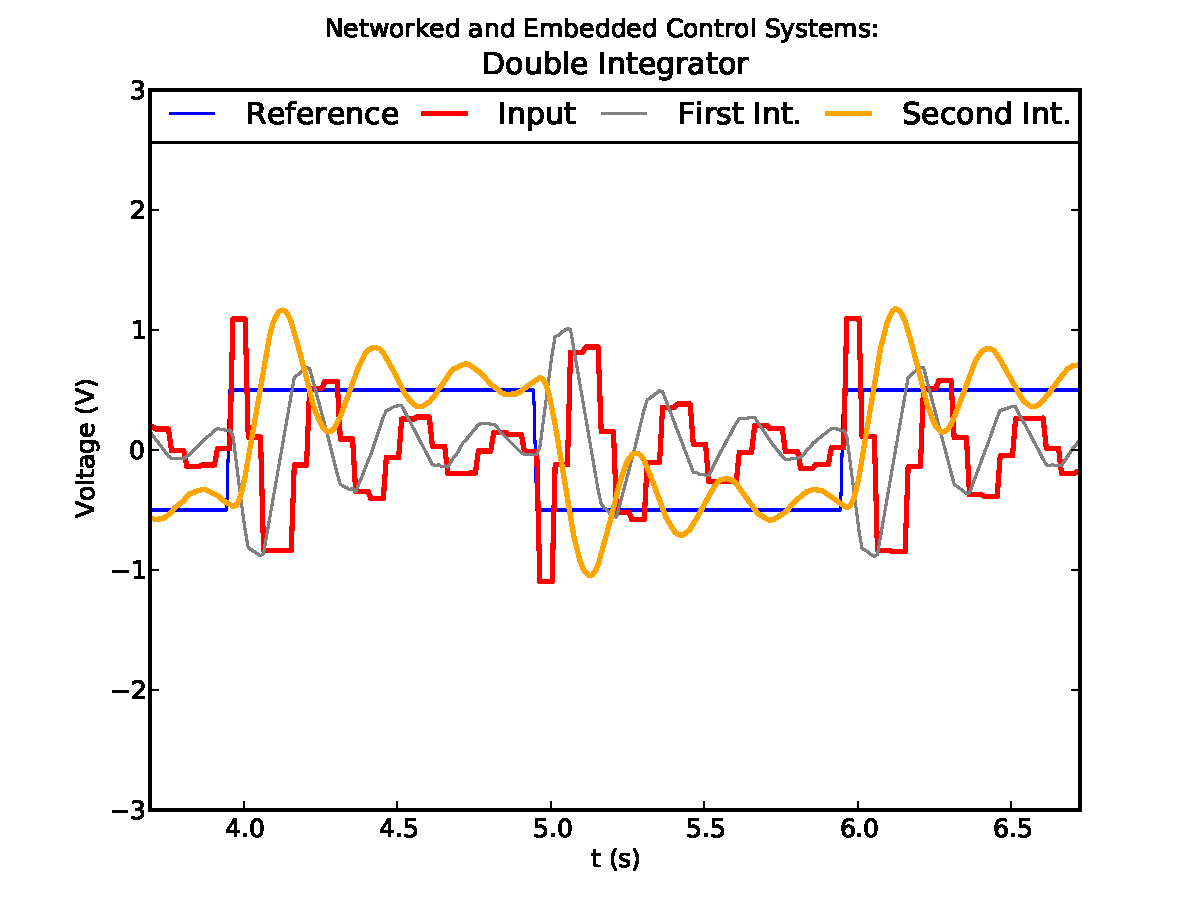
\includegraphics[width=0.85\linewidth]{necs_di_graph}
%	}
%	\\
%	\subfloat[Amb el bus CAN saturat de missatges, amb textos en català, només amb línies de referència i segona integral i en format PDF.]{\label{di_saturat_ref_segona_cat}
%		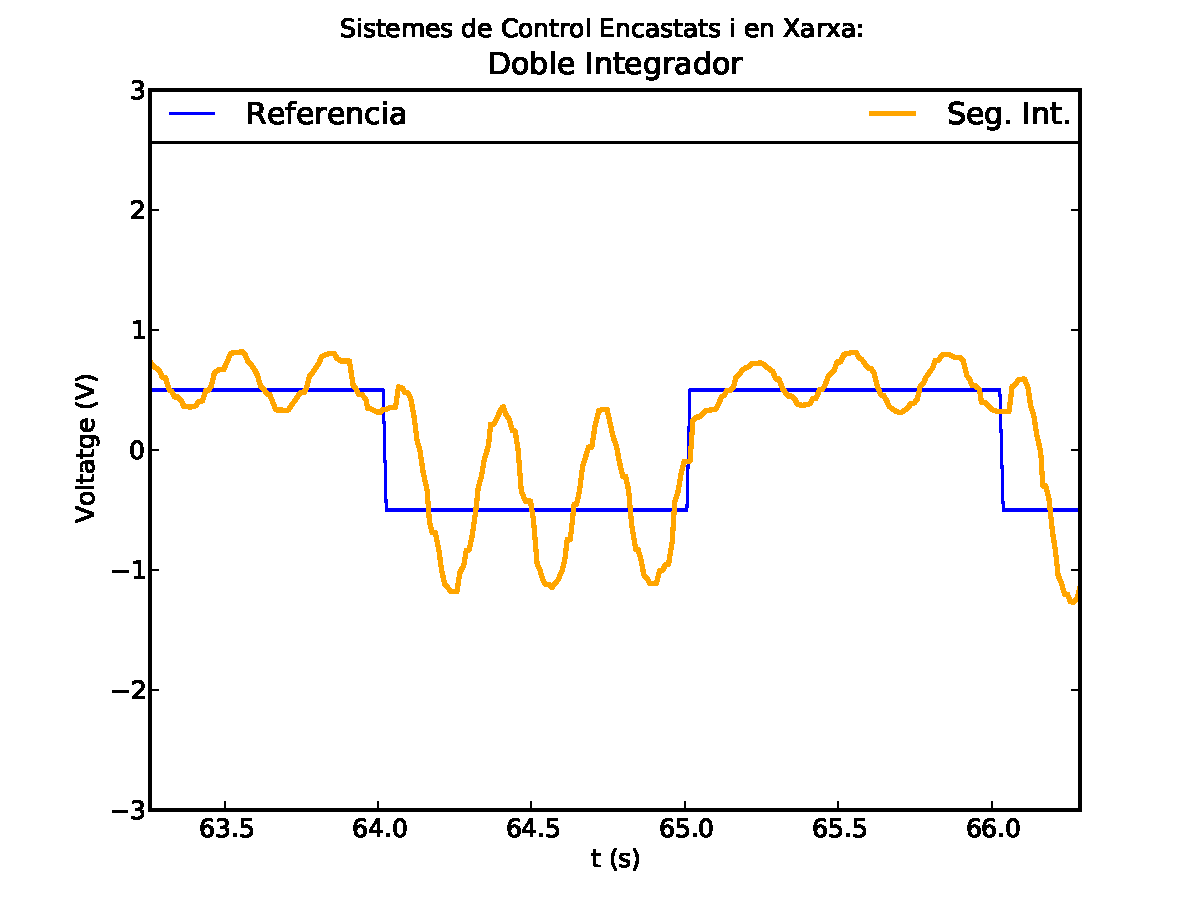
\includegraphics[width=0.85\linewidth]{di_saturat_ref_segona_cat}
%	}

%	\caption[Diferents gràfiques generades amb el programa \DCSMonitor]{Diferents gràfiques generades amb el programa \DCSMonitor del control d'un doble integrador.}
%    \label{fig:comparacio:graph}
%\end{figure}


%\begin{figure}[tbp]
%\centering
%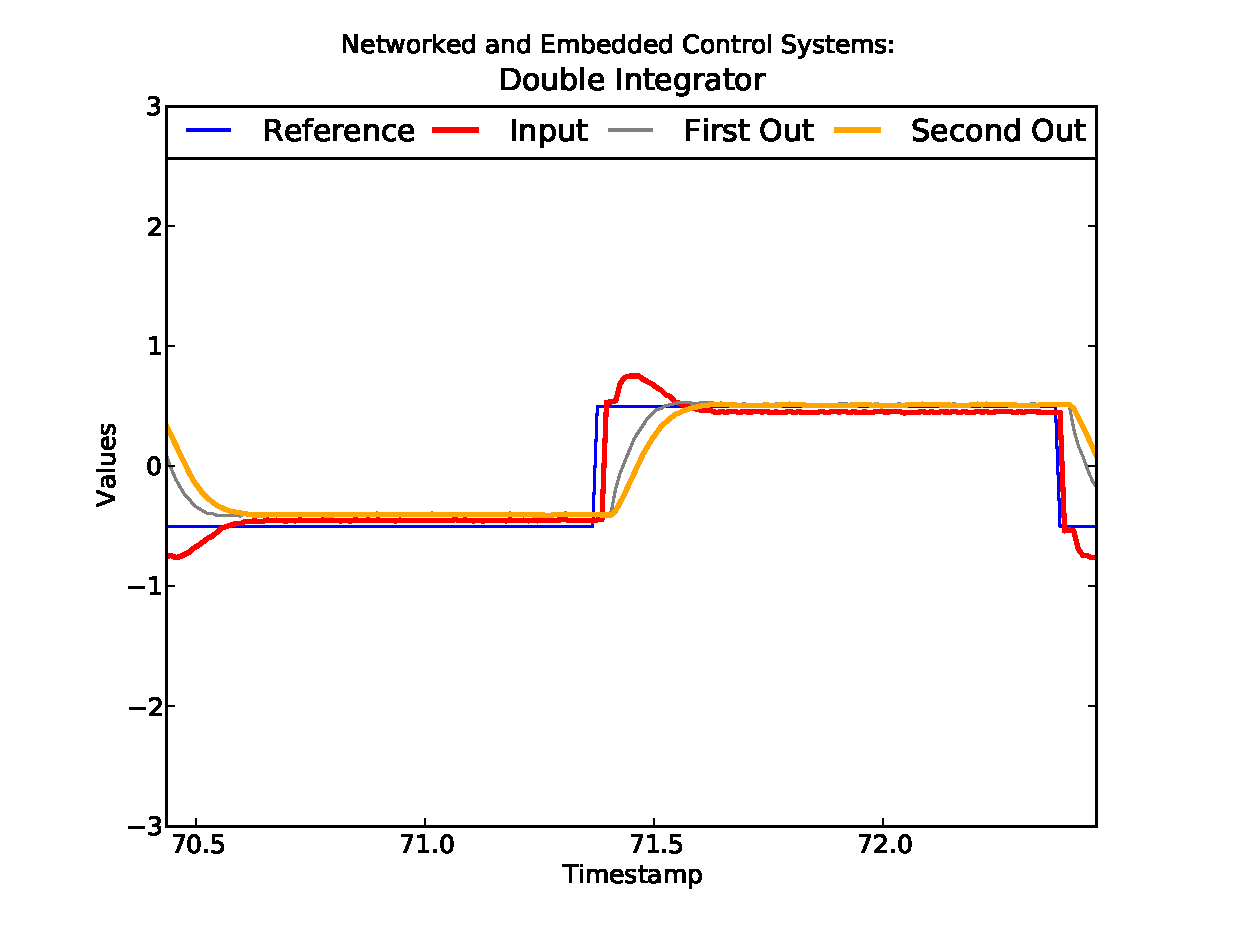
\epsfig{file=grup_12_eps.eps,width=0.9\linewidth,clip=}
%\caption{A title of some sort}
%\label{fig:aNicePicture}
%\end{figure}

%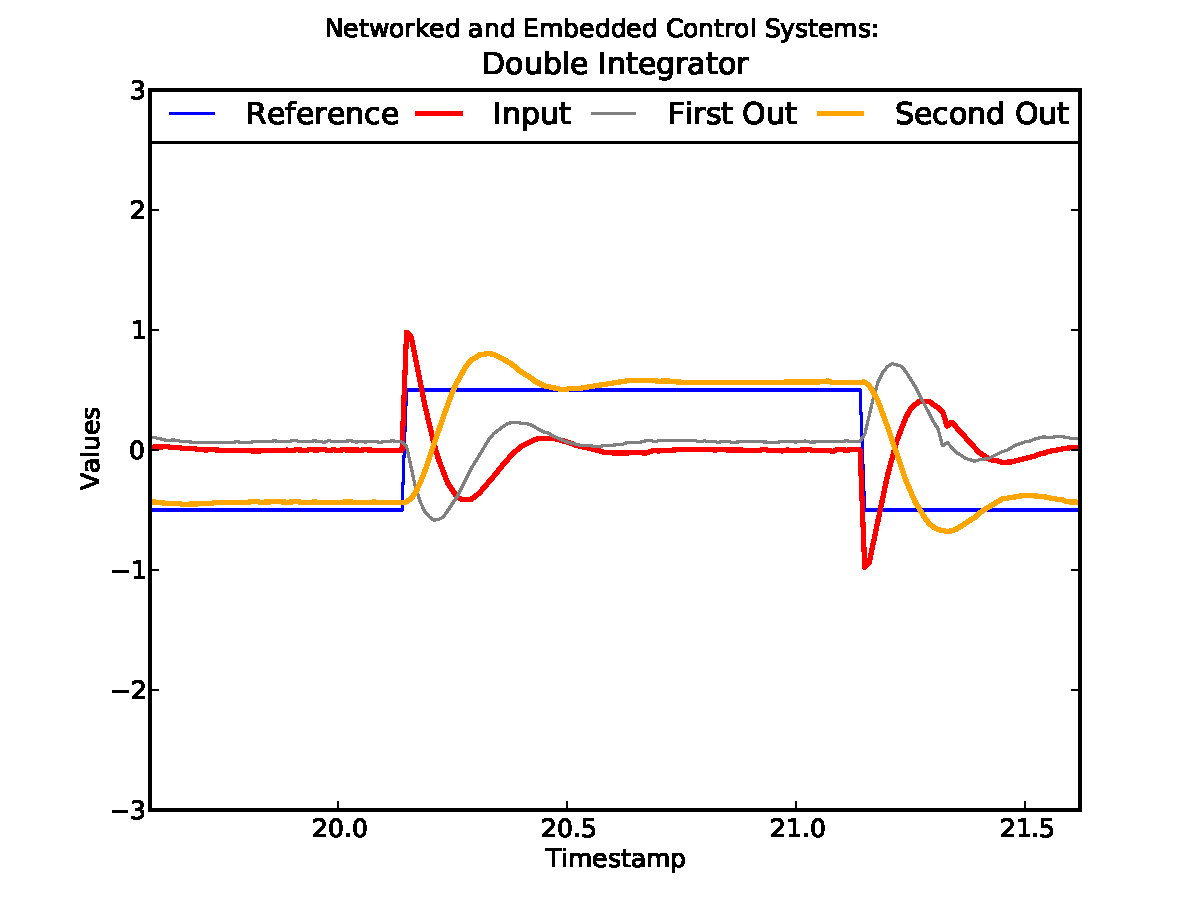
\includegraphics{3_laboratory_design/figures/grup_1_pdf.pdf}


%====================================================================================%
% Idiomes
%====================================================================================%
\subsection{Idiomes}\label{cap:dis:idi}

Un dels requisits que es buscava complir en el nou laboratori era que el programa visual fos multilingüe per tal de poder ser distribuït més fàcilment podent realitzar el laboratori en diferents parts del món.

Per tant es va estudiar la manera de realitzar aquest requisit de forma escalable i que fos ampliable fàcilment. Així que es va trobar una combinació de programes que podien realitzar aquesta tasca d'aquesta manera.

\begin{itemize}
	\item PyQT4 : Amb aquesta llibreria de \Python podem crear tot l'entorn visual del programa \DCSMonitor, i també ens permetrà fer la integració de les gràfiques (referent al idioma veure capítol \ref{cap:imp:idi:pyqt4}).
	\item Pylupdate4 : Amb aquest programa podrem generar fitxers entendibles per QtLingüist per tal de traduir tots els textos  que vulguem del programa (veure capítol \ref{cap:imp:idi:pylupdate4}).
	\item QtLingüist : Amb aquest programa es poden editar fàcilment els fitxers generats amb Pylupdate4, i un cop traduïts es genera un fitxer que la llibreria PyQT4 podrà interpretar en temps d'execució (veure capítol \ref{cap:imp:idi:qtlinguist})
\end{itemize}

Gràcies a totes aquestes eines el programa \DCSMonitor (que s'executa a l'ordinador) serà capaç de mostrar la informació essencial en varis idiomes, i és fàcilment ampliable ja que s'ha realitzat de forma estructurada per tal que seguint algunes instruccions es puguin generar més idiomes.

Actualment està traduït en els següents idiomes, però la llista pot ser fàcilment ampliada:

\begin{itemize}
	\item Català
	\item Espanyol
	\item Anglès
	\item Francès
\end{itemize}


%====================================================================================%
% Conclusions
%====================================================================================%
\section{Conclusions}\label{cap:dis:conc}

Al llarg d'aquest capítol hem pogut veure més profundament de que tracta el laboratori actual, i en quins punts es quedava curt. Tot seguit hem proposat un entorn en el que tots els llaços de control estiguessin en el mateix bus, i d'aquesta manera hem vist que necessitàvem dissenyar un ordre d'identificadors CAN que solucionessin els conflictes entre dispositius. Així que hem creat identificadors de missatges CAN amb alta prioritat per poder mantenir els controls més estables, i missatges en canvi menys prioritaris, que s'ocuparan exclusivament d'ocupar la resta del bus, sense perjudicar en cap moment el control.

També hem organitzat els diferents senyals de comunicació serie per RS232 per poder demanar l'execució de diferents accions al dispositiu \Monitor, i quin tipus d'accions volem que aquest sigui capaç de realitzar.

Amb tot això ven clar hem pogut dissenyar la interfície del programa \DCSMonitor, que ens ha de proporcionar informació de manera fàcil, i poder interactuar amb ell de manera intuïtiva.

Hem pogut veure mètodes per generar les gràfiques del control en temps real, i la seva exportació en diversos formats.

I per finalitzar hem vist que podem realitzar el programa \DCSMonitor multilingüe amb la utilització de varis programes, i seguint un cert ordre en la obtenció dels fitxers de traducció finals.

Ara que ja hem pogut veure la fase de disseny es l'hora d'implementar tots els sistemes, aquesta part es una de les més llargues, ja que moltes de les eines a utilitzar són noves i fer tasques senzilles poden comportar temps llargs. El que es veurà en la següent secció es el resultat de la implementació de tota la fase de disseny que hem vist. I algunes captures del programa final.
